\paragraph{QuizziPedia::Front-End::ModelViews::QuizEventModelView}
							
\label{QuizziPedia::Front-End::ModelViews::QuizEventModelView}

\begin{figure}[ht]
	\centering
	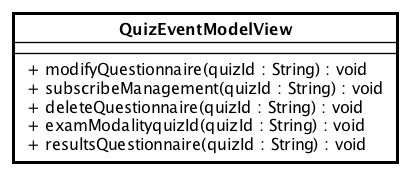
\includegraphics[scale=0.5,keepaspectratio]{UML/Classi/Front-End/QuizziPedia_Front-end_ModelView_QuizEventModelView.png}
	\caption{QuizziPedia::Front-End::ModelViews::QuizEventModelView}
\end{figure} \FloatBarrier

\begin{itemize}
	\item \textbf{Descrizione}: classe di tipo modelview la cui istanziazione è contenuta all'interno della variabile di ambiente \texttt{\$scope} di \textit{Angular\ped{G}}. All'interno di essa sono presenti le variabili e i metodi necessari per il \textit{Two-Way Data-Binding\ped{G}} tra le \textit{directives\ped{G}}\\ \texttt{EliminationAndModifyDirective}, \texttt{ExamModalityDirective} e \\\texttt{QuestionnaireResultsDirective} e il \textit{controller\ped{G}} \texttt{QuizEventController};
	\item \textbf{Utilizzo}: viene utilizzata per effettuare il \textit{Two-Way Data-Binding\ped{G}} tra le \textit{directives\ped{G}}\\ \texttt{EliminationAndModifyDirective}, \texttt{ExamModalityDirective} e \\\texttt{QuestionnaireResultsDirective} e il \textit{controller\ped{G}} \texttt{QuizEventController} rendendo disponibili variabili e metodi;
	\item \textbf{Relazioni con altre classi}: 
	\begin{itemize}
		\item \textbf{OUT \texttt{EliminationAndModifyDirective}}: componente grafico contenente i bottoni per eliminare o modificare un questionario;
		\item \textbf{OUT \texttt{ExamModalityDirective}}: \textit{directive\ped{G}} contenente i componenti grafici per attivare la modalità esame su un questionario e gestire le iscrizioni; 
		\item \textbf{OUT \texttt{QuestionnaireResultsDirective}}: rappresenta il componente grafico che permette all'utente autenticato pro di vedere i risultati di chi ha compilato il questionario. Tale componente è contenuto nella lista dei questionari abilitati alla compilazione. \'E possibile accedere alla lista dei risultati azionando l'evento ad esso collegato; 
		\item \textbf{OUT \texttt{QuizEventController}}: questa classe permette di reagire ai comandi dell'utente durante la gestione dei suoi questionari.
	\end{itemize}
	\item \textbf{Metodi}: 
	\begin{itemize}
		\item \texttt{+ modifyQuestionnaire(quizId: String): void} \\
		Metodo che gestisce l'evento click sul pulsante di modifica questionario. Effettua il redirect alla pagina di gestione questionari.\\
		\textbf{Parametri}:
		\begin{itemize}
			\item \texttt{quizId: String}\\ 
			Parametro che indica l'identificativo univoco di un questionario.
		\end{itemize}
		\item \texttt{+ deleteQuestionnaire(quizId: String): void} \\
		Metodo che gestisce l'evento click sul pulsante di eliminazione questionario. Effettua il redirect alla pagina di gestione questionari.\\
		\textbf{Parametri}:  
		\begin{itemize}
			\item \texttt{quizId: String}\\
			Parametro che indica l'identificativo univoco di un questionario.
		\end{itemize}
		
		\item \texttt{+ subscribeManagement(quizId: String): void} \\
		Metodo che gestisce l'evento click sul pulsante di gestione iscrizioni. Effettua il redirect alla pagina di gestione iscrizioni.\\
		\textbf{Parametri}:
		\begin{itemize}
			\item \texttt{quizId: String}\\
			Parametro che indica l'identificativo univoco di un questionario.
		\end{itemize}
		
		\item \texttt{+ examModalityquizId: String(): void} \\
		Metodo che gestisce l'evento click sul pulsante di attivazione modalità esame. Effettua il redirect alla pagina di gestione questionari.
		\textbf{Parametri}:
		\begin{itemize}
			\item \texttt{quizId: String}\\ 
			Parametro che indica l'identificativo univoco di un questionario.
		\end{itemize}
		\item \texttt{+ resultsQuestionnaire(quizId: String): void} \\
		Metodo che gestisce l'evento click sul pulsante di allenamento. Effettua il redirect alla pagina di gestione questionari.
		\begin{itemize}
			\item \texttt{quizId: String}\\
			Parametro che indica l'identificativo univoco di un questionario.
		\end{itemize}   
	\end{itemize}
\end{itemize}